\documentclass[11pt, oneside]{article}   	% use "amsart" instead of "article" for AMSLaTeX format
\usepackage{geometry}                		% See geometry.pdf to learn the layout options. There are lots.
\geometry{letterpaper}                   		% ... or a4paper or a5paper or ... 
%\geometry{landscape}                		% Activate for for rotated page geometry
%\usepackage[parfill]{parskip}    		% Activate to begin paragraphs with an empty line rather than an indent
\usepackage{graphicx}				% Use pdf, png, jpg, or eps� with pdflatex; use eps in DVI mode
								% TeX will automatically convert eps --> pdf in pdflatex		
\usepackage{amssymb}
\usepackage{amsmath}
\usepackage{parskip}
\usepackage{color}
\usepackage{hyperref}

\title{Using the Cauchy residue theorem}
%\author{The Author}
%\section{}
%\subsection*{}
\date{}							% Activate to display a given date or no date

\graphicspath{{/Users/telliott_admin/Dropbox/Tex/png/}}
% \begin{center} 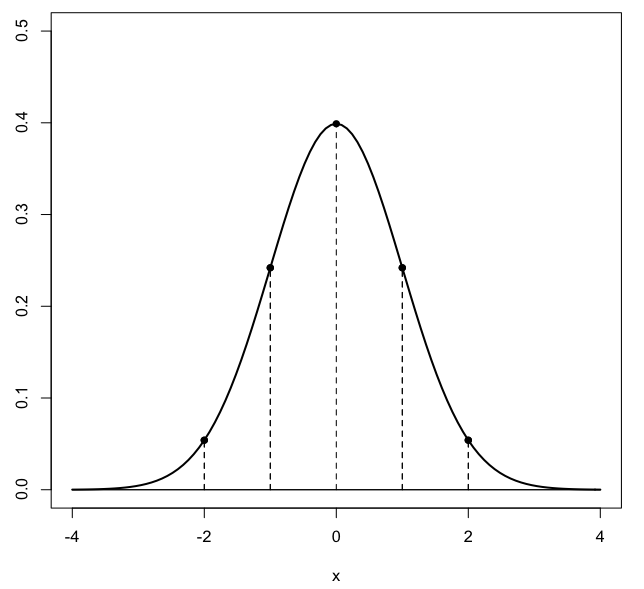
\includegraphics [scale=0.4] {gauss3.png} \end{center}
\begin{document}
\maketitle
\Large
Much of the challenge in converting an integral over the real numbers into a complex integral is setting up an appropriate integral and region of the complex plane.

For any point $z$, its complex conjugate $z*$ is the reflection of the point across the $x$-axis and so if
\[ z = x + iy \]
then
\[ z* = x - iy \]
\[ z + z* = 2x \]
\[ z - z* = 2iy \]
Consider the points $z$ on the unit circle.  The curve that goes all the way around is of course $\theta = 0 \rightarrow 2\pi$.  And the sine and cosine of the angle are the values of $x$ and $y$ for some particular $z$ so
\[ \cos \theta = \frac{1}{2} (z + z*) \]
Recall that for $z$ with unit length the inverse (and other powers) of $z$ also lie on the unit circle.  Thus:
\[ \frac{1}{z} = \frac{z*}{zz*} = \frac{z*}{r^2} = z* \]
and so 
\[ \cos \theta = \frac{1}{2} (z + z*) = \frac{1}{2} (z + \frac{1}{z}) \]
For this set of values (the unit circle), we can write 
\[ z = re^{i\theta} = e^{i\theta} \]
\[ \frac{dz}{d\theta} = i e^{i\theta} = iz \]
\[ \frac{1}{iz} \ dz = d \theta \]
So if we have the real integral
\[ \int_0^{2\pi} \cos \theta \ d \theta \]
we can write it as
\[ \oint \frac{1}{2} (z + \frac{1}{z}) \ \frac{1}{iz} \ dz = \frac{1}{2i} \oint 1 + \frac{1}{z^2} \ dz \] 
The first integral of the first integrand is zero, but the second one has a residue at the origin although of course the value must be zero too since
\[ \int_0^{2\pi} \cos \theta \ d \theta = 0 \]

Let us move on to the example given in my source:
\[ \int_0^{2\pi} \frac{1}{1 + a \cos \theta} \ d \theta, \ \ \ -1 < a < 1 \]
Substituting as above we get
\[ \oint \frac{1}{1 + \frac{a}{2}(z + \frac{1}{z})} \ \frac{1}{iz} \ dz \]
\[ = \frac{2}{i} \oint \frac{1}{2z + az^2 + a} \ dz \]
We need to find the poles.  These are where
\[ 2z + az^2 + a = 0 \]
Using the quadratic formula:
\[ z_{\pm} = \frac{-2 \pm \sqrt{4-4a^2}}{2a} = \frac{1}{a} ( -1 \pm \sqrt{1-a^2}) \]
Only the positive root is inside the unit circle, so
\[ z_0 =  \frac{1}{a} ( -1 + \sqrt{1-a^2}) \]
And according to the source what we do is to write the integrand as a ratio of functions:
\[ \frac{g}{h} = \frac{2}{i} \frac{1}{(az^2 + 2z + a)} \]
The residue is 
\[ \frac{g}{h'} =  -\frac{2}{i} \ \frac{1}{(az^2 + 2z + a)^2} (2az + 2) \]
evaluated at $z_0$.

The residue is given as
\[ R_{+} = \frac{1}{i} \ \frac{1}{\sqrt{1-a^2}} \]
and the answer is then
\[ I = 2 \pi i R_+ = \frac{2 \pi}{\sqrt{1-a^2}} \]

\end{document}  
